\chapter{Огляд та затягнутий вступ}

\section{Історія}

Ідея латинських квадратів породжується якнайменше 300 років тому у монограмі \emph{Koo-Soo-Ryak}, яку написав Choi Seok-Jeong (1646-1715). 
Він використовував ортогональні латинські квадрати 9 порядку для побудови магічних квадратів. У своїх нотатках він зауважив, що не міг знайти ортогональні латинські квадрати 10 порядку.

Але це не перша поява латинських квадратів. Існують амулети латинських квадратів середньовічного Ісламу, магічний квадрат аль-Буні. Вони доказують, що люди того часу знали мінімум 2 ортогональні латинські квадрати розміру $4\times 4$.

Тобто все ж невідоме точне походження латинських квадратів.

У 1776 році Ойлер презентував роботу \emph{De Quadratis Magicis} Академії Наук в Петербурзі. Там він показав побудову магічних квадратів порядку 3, 4, 5 з ортогональних квадратів. Також він продемонстрував проблему щодо магічного квадрату порядку 6, яка відома як \emph{Euler's 36 Officers Problem}. Надалі Ейлер припускав, що не існує таких рішень для порядку 6, та навіть пішов далі --- не існує ортогональних латинських квадратів порядку $n \equiv 2 (\operatorname{mod} 4)$.

Але його останнє припущення було спростовано 1958 року Раджом Бозе та Шарадчандром Шрікханде, які побудували два ортогональні латинські квадрати 22 порядку. Далі у 1960 році вони дізналися, що два ортогональні латинські квадрати порядку $n$ існують для всіх $n \equiv 2(\operatorname{mod} 4)$, окрім 2 та 6.


\section{Латинські квадрати та часткові латинські квадрати}

\begin{definition}
    Латинський квадрат порядку $n$ це матриця $L$ розміру $n \times n$ з елементами із множини $\set{1, \dots, n}$, де кожен елемент зустрічається у кожному рядку та колонці лише один раз.
\end{definition}

\begin{align*}
    L_{4,0} = \begin{bmatrix}
        0 & 1 & 2 & 3 \\
        3 & 0 & 1 & 2 \\
        2 & 3 & 0 & 1 \\
        1 & 2 & 3 & 0
    \end{bmatrix} 
    \;\; & \;\;
    L_{3,0} = \begin{bmatrix}
        1 & 0 & 2 \\
        0 & 2 & 1 \\
        2 & 1 & 0
    \end{bmatrix}
\end{align*}

Одне з найбільших досліджень латинських квадратів стосується часткових латинських квадратів.

\begin{definition}
    Частковий латинський квадрат порядку $n$ це матриця $P$ розміру $n \times n$, де кожне місце або пусте, або містить елемент із множини $\set{1, \dots, n}$ з умовою, що кожний елемент зустрічається у кожному рядку (колонці) лише один раз.
\end{definition}

Одне з важливих досліджень латинських квадратів розпочав Маршалл Голл та Герберт Джон Райзер. Воно стосується характеризації часткових латинських квадратів. Вже останні можуть бути доповнені до латинських квадратів без додавання рядків, колонок чи елементів. 

\begin{figure}[ht]
    \begin{subfigure}[b]{0.5\textwidth}
        \centering
        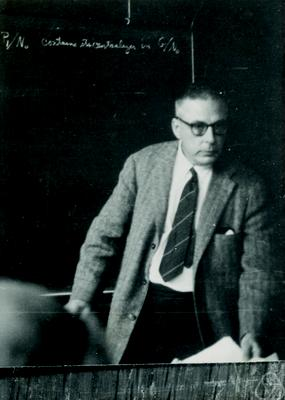
\includegraphics[scale=0.3]{Images/Marshall_Hall.jpg}
        \caption*{Маршалл Голл}
    \end{subfigure}
    \begin{subfigure}[b]{0.5\textwidth}
        \centering
        
\includegraphics[scale=0.4]{Images/Herbert_Ryser.jpg}
        \caption*{Герберт Райзер}
    \end{subfigure}
\end{figure}

